\documentclass{article}
\usepackage{amsfonts}
\usepackage{amsmath}
\usepackage{amsthm}
\usepackage[utf8]{inputenc}
\usepackage{braket}

% Vector
\newcommand*\mat[1]{ \begin{pmatrix} #1 \end{pmatrix}}
\newcommand*\arr[1]{ \begin{bmatrix} #1 \end{bmatrix}}

\newcommand*\V[1]{ \boldsymbol{#1}}

% Apartado de un ejemplo
\theoremstyle{definition}
\newtheorem{ejemplo}{Ejemplo}[section]

% Gráficos con tikz
\usepackage{tikz}

\usetikzlibrary{calc,fadings,decorations.pathreplacing}
\usetikzlibrary{backgrounds,fit}
\newcommand\pgfmathsinandcos[3]{%
  \pgfmathsetmacro#1{sin(#3)}%
  \pgfmathsetmacro#2{cos(#3)}%
}
\newcommand\LongitudePlane[3][current plane]{%
  \pgfmathsinandcos\sinEl\cosEl{#2} % elevation
  \pgfmathsinandcos\sint\cost{#3} % azimuth
  \tikzset{#1/.estyle={cm={\cost,\sint*\sinEl,0,\cosEl,(0,0)}}}
}
\newcommand\LatitudePlane[3][current plane]{%
  \pgfmathsinandcos\sinEl\cosEl{#2} % elevation
  \pgfmathsinandcos\sint\cost{#3} % latitude
  \pgfmathsetmacro\yshift{\cosEl*\sint}
  \tikzset{#1/.estyle={cm={\cost,0,0,\cost*\sinEl,(0,\yshift)}}} %
}
\newcommand\DrawLongitudeCircle[2][1]{
  \LongitudePlane{\angEl}{#2}
%  \tikzset{current plane/.prefix style={scale=#1}}
   % angle of "visibility"
  \pgfmathsetmacro\angVis{atan(sin(#2)*cos(\angEl)/sin(\angEl))} %
  \draw[current plane] (\angVis:1) arc (\angVis:\angVis+180:1);
  \draw[current plane,dashed] (\angVis-180:1) arc (\angVis-180:\angVis:1);
}
\newcommand\DrawLatitudeCircle[2][1]{
  \LatitudePlane{\angEl}{#2}
%	\tikzset{current plane/.prefix style={scale=#1}}
  \pgfmathsetmacro\sinVis{sin(#2)/cos(#2)*sin(\angEl)/cos(\angEl)}
  % angle of "visibility"
  \pgfmathsetmacro\angVis{asin(min(1,max(\sinVis,-1)))}
  \draw[current plane] (\angVis:1) arc (\angVis:-\angVis-180:1);
  \draw[current plane,dashed] (180-\angVis:1) arc (180-\angVis:\angVis:1);
}

%% document-wide tikz options and styles

%\tikzset{%
%  >=latex, % option for nice arrows
%  inner sep=0pt,%
%  outer sep=2pt,%
%  mark coordinate/.style={inner sep=0pt,outer sep=0pt,minimum size=3pt,
%    fill=black,circle}%
%}

\begin{document}

%\tableofcontents

\section{Introducción a la computación cuántica}
\subsection{Preliminares}
La computación cuántica es un nuevo paradigma de computación, que busca la
resolución de problemas empleando las propiedades de la mecánica cuántica.

Fundamenta su utilidad en el hecho de que algunos problemas que tienen una alta
complejidad en los ordenadores clásicos, y son intratables, pasan a ser
tratables en un ordenador cuántico.

\subsection{El qbit}
Un bit, definido como la unidad básica de información, tan sólo puede 
encontrarse en un estado, de entre dos posibles. Sea $y$ un bit, $y \in 
\{0,1\}$.

La forma en la que se implementa un bit depende de la arquitectura: la posición 
de una leva mecánica en la máquina de Babagge, la presencia o ausencia de un 
agujero en una tarjeta perforada, anillos de ferrita que se magnetizan en un 
sentido o en otro, dos niveles de voltaje diferentes...
Todas estas representaciones, diferentes en su naturaleza, comparten una 
propiedad en común; es posible escribir un estado, y posteriormente realizar una 
lectura. Esta sencilla operación es la base para toda computación.

Un bit probabilístico, se encuentra en un estado $x$ determinado, de forma que 
al medirlo se obtiene un bit clásico $y$. La probabilidad de obtener un 0, es 
$a$, y de obtener un 1 es $b$, y ambas suman 1: $a + b = 1$.
$$p(y = 0) = a, \quad p(y = 1) = b, \quad a,b \in [0, 1]$$
De esta forma, se pueden representar en un vector, las probabilidades de que al 
medir $x$ se obtenga un 0 o un 1:
$$ x = \mat{a \\ b}, \quad x_0 = a, \quad x_1 = b$$
La suma total de las probabilidades de $x$ debe ser 1, $\sum x_i = 1$. Además $x 
\in \mathbb{R}^2$, cuyas componentes $x_i \in [0,1]$.
Por ejemplo, lanzar una moneda al aire, se corresponde con una variable 
aleatoria de probabilidad igual para ambos estados:
$$ x = \mat{0.5 \\ 0.5} $$
Sin embargo, tras el lanzamiento, al observar el resultado, tan sólo puede ser 
cara o cruz, esto es, 0 o 1.
Un bit clásico es un caso particular de un bit probabilístico:
$$ \text{bit}_0 = \mat{1\\0}, \quad \text{bit}_1 = \mat{0\\1} $$
Un qbit o bit cuántico, es similar al bit probabilístico, pero con algunas 
diferencias. Para representar un estado se emplea también un vector $z$:
$$ z = \mat{\alpha \\ \beta}$$
Al medir $z$ se obtendrá un bit clásico $y$, de igual modo que en el bit 
probabilístico, pero la probabilidad es diferente:
$$p(y=0) = |\alpha|^2, \quad p(y=1) = |\beta|^2$$
La probabilidad de que salga 0 o 1 debe seguir sumando la unidad, por lo que 
$|\alpha|^2 + |\beta|^2 = 1$. Pero en el caso del qbit $\alpha, \beta \in 
\mathbb{C}$. Un bit probabilístico es también un caso particular de un qbit, 
cuando $a = |\alpha|^2$ y $b = |\beta|^2$:
$$ x = \mat{|\alpha|^2 \\ |\beta|^2}$$

%\begin{figure}
%\begin{minipage}[b][6cm]{0.3\linewidth}
%\subfloat[A]{\includegraphics[width=3cm,height=2cm]{logo}}
%
%\vfill
%\subfloat[B]{\includegraphics[width=3cm,height=2cm]{logo}}
%\end{minipage}%
%\begin{minipage}[t][6cm]{0.3\linewidth}
%\subfloat[D]{\includegraphics[width=3cm,height=6cm]{logo}}
%\end{minipage}%
%\begin{minipage}[t][6cm]{0.3\linewidth}
%\subfloat[D]{\includegraphics[width=3cm,height=6cm]{logo}}
%\end{minipage}
%\caption{Many figures}\label{foo}
%\end{figure}
%
%
%\begin{figure}[h]
%\begin{center}
%\begin{tikzpicture}
%	\coordinate (S) at (0,0);
%	\coordinate (E) at S+(3,0);
%	\coordinate (M1) at (E);
%	\coordinate (M0) at (3,-0.5);
%	\draw [dotted] (S) -- (E);
%	\draw[->] (M0) -- (M1);
%
%\end{tikzpicture}
%\end{center}
%\caption{Bit clásico}
%\label{fig:bit_clasico}
%\end{figure}
%
%
%\begin{tikzpicture}
%	\draw (0,0) -- (3,0);
%	\draw [fill] (2,0) circle [radius=0.1];
%
%
%\end{tikzpicture}
%
%
%\begin{figure}[ht]
%\begin{center}
%\begin{tikzpicture} % MERC
%
%% Stereographic and cylindrical map projections
%% Author: Tomasz M. Trzeciak
%% Source: LaTeX-Community.org 
%%         <http://www.latex-community.org/viewtopic.php?f=4&t=2111>
%
%%% some definitions
%
%\def\R{1} % sphere radius
%\def\angEl{25} % elevation angle
%\def\angAz{-130} % azimuth angle
%\def\angPhiOne{-40} % longitude of point P
%\def\angPhiTwo{0} % longitude of point Q
%\def\angBeta{60} % latitude of point P and Q
%
%%% working planes
%
%\pgfmathsetmacro\H{\R*cos(\angEl)} % distance to north pole
%\LongitudePlane[xzplane]{\angEl}{\angAz}
%\LongitudePlane[pzplane]{\angEl}{\angPhiOne}
%\LongitudePlane[qzplane]{\angEl}{\angPhiTwo}
%\LatitudePlane[equator]{\angEl}{0}
%
%%% draw background sphere
%
%%\fill[ball color=white] (0,0) circle (\R); % 3D lighting effect
%%\fill[white] (0,0) circle (\R); % just a white circle
%\draw (0,0) circle (\R);
%
%%% characteristic points
%
%\coordinate[mark coordinate] (O) at (0,0);
%\coordinate[mark coordinate] (N) at (0,\H);
%\coordinate[mark coordinate] (S) at (0,-\H);
%\path[xzplane] (\R,0) coordinate (XE);
%\path[pzplane] (\angBeta:\R) coordinate (P);
%\path[pzplane] (\R,0) coordinate (PE);
%\path[qzplane] (\angBeta:\R) coordinate (Q);
%\path[qzplane] (\R,0) coordinate (QE);
%
%%% meridians and latitude circles
%
%\DrawLongitudeCircle[\R]{\angAz} % xzplane
%\DrawLongitudeCircle[\R]{\angAz+90} % yzplane
%%\DrawLongitudeCircle[\R]{\angPhiOne} % pzplane
%%\DrawLongitudeCircle[\R]{\angPhiTwo} % qzplane
%%\DrawLatitudeCircle[\R]{\angBeta}
%\DrawLatitudeCircle[\R]{0} % equator
%
%% shifted equator in node with nested call to tikz 
%% (I didn't know it's possible)
%%\node at (0,1.6*\R) { \tikz{\DrawLatitudeCircle[\R]{0}} };
%
%%% draw lines and put labels
%
%%\draw (-\R,-\H) -- (-\R,2*\R) (\R,-\H) -- (\R,2*\R);
%%\draw[->] (O) -- +(0,1.5*\R) node[above] {$|0\rangle$};
%%\node[above=8pt] at (N) {$|0\rangle$};%{$\mathbf{N}$};
%%\node[below=8pt] at (S) {$|1\rangle$};%{$\mathbf{S}$};
%%\node[right=8pt] at (P) {$|\Phi \rangle$};
%\draw[->] (O) -- (P);
%%\draw[dashed] (O) -- (N);
%%\draw[dashed] (XE) -- (O) -- (PE);
%%\draw[dashed] (O) -- (QE);
%%\draw[pzplane,->,thin] (0:0.5*\R) to[bend right=15]
%%    node[midway,right] {$\beta$} (\angBeta:0.5*\R);
%%\path[pzplane] (0.5*\angBeta:\R) ;%node[right] {$\hat{1}$};
%%\path[qzplane] (0.5*\angBeta:\R) ;%node[right] {$\hat{2}$};
%%\draw[equator,->,thin] (\angAz:0.5*\R) to[bend right=30]
%%		node[pos=0.4,above] {$\phi$} (\angPhiOne:0.5*\R);
%%\draw[pzplane,->,thin] (90:0.5*\R) to[bend left=30]
%%		node[midway,right] {$\theta$} (\angBeta:0.5*\R);
%%\draw[equator,->] (-90:\R) arc (-90:-70:\R) ;%node[below=0.3ex] {$x = a\phi$};
%%\path[xzplane] (0:\R) node[below] {$\theta=0$};
%%\path[xzplane] (\angBeta:\R);% node[below left] {$\beta=\beta_0$};
%
%\end{tikzpicture}
%\end{center}
%\caption{Bloch Sphere}
%\label{25:fig:bloch_sphere}
%\end{figure}

\subsection{Múltiples qbits}
Para representar $N$ bits, es suficiente con un vector $\boldsymbol{b} = 
\mat{b_0 & b_1 & \cdots & b_{N-1} }^T$. De forma que $b_i \in \{0,1\}$. Por 
ejemplo un byte, que está formado de 8 bits, es:
$$\mat{b_0 & b_1 & b_2 & b_3 & b_4 & b_5 & b_6 & b_7}^T$$
Simplificando la notación, representando solo los bits:
$$\boldsymbol{b} = b_0 \, b_1 \, b_2 \, b_3 \, b_4 \, b_5 \, b_6 \, b_7$$
Por lo que $\boldsymbol{b} \in \{0,1\}^N$, y numerando cada vector con:
$$d = \sum_i 2^i b_i$$
Por ejemplo $d=14$ es $\boldsymbol{b} = 1110$ con $N=4$. $1110_b = 14_d$
Por ejemplo $11000001_b = 193_d$


\subsection{Operaciones}



Para realizar una operación sobre un estado cuántico, se emplea un operador 
expresado por una matriz.

Por ejemplo, la puerta NOT que invierte el estado de un bit, tiene una operación 
análoga en la computación cuántica.
%
$$ NOT = \mat{0 & 1 \\ 1 & 0} $$
%
De modo que al aplicarla sobre un estado $\ket{\psi} = \mat{\alpha & \beta}^T$, 
se obtiene:
%
$$ NOT \ket{\psi} = \mat{0 & 1 \\ 1 & 0} \mat{\alpha \\ \beta} = \mat{\beta \\ 
\alpha} $$
%
Las amplitudes se han invertido, de forma análoga a un estado clásico. Si 
$\ket{\psi} = \ket{0}$, entonces $NOT\ket{0} = NOT \mat{1 & 0}^T = \mat{0 & 
1}^T = \ket{1}$. Y de igual forma para $NOT \ket{1} = \ket{0}$.

\newpage

\section{Simulación de un circuito cuántico}
\subsection{Estructuras de datos}
La representación de los estados cuánticos así como los operadores, se realiza
mediante matrices huecas. La clase \texttt{Qobj} de QuTiP permite emplear de
forma implícita las matrices huecas de \texttt{scipy.sparse}.

De esta forma, un estado $\ket{\phi_0} = \ket{000} $

\newpage

Dado un $s$, la ecuación $s \cdot y = 0$ con $s, y \in \mathbb Z_2^n$ tiene 
varias soluciones para $y$.
$$ s \cdot y = s_0 \cdot y_0 + s_1 \cdot y_1 + \ldots + s_{n-1} \cdot y_{n-1} = 
\sum_{i}{s_i \cdot y_i} = 0$$
Si $s = 0$, entonces existen $2^n$ soluciones, dado que $s_i = 0$, y cualquier 
valor para $y$ satisface la ecuación.
$$ \sum_{i}{s_i \cdot y_i} = \sum_{i}{0 \cdot y_i} $$

$$ s_i \cdot y_i = 0 \cdot y_i = 0 \cdot 0 = 0 \cdot 1 = 0 = s_i$$
Si $s \neq 0$, entonces las posibles soluciones se reducen, ya que en algún caso 
$s_i = 1$, por lo que $s_i \cdot y_i = 1 \cdot y_i = y_i$.
En el caso en el que el número de unos en $s$ sea uno, para un $i$, $s_i = 1$, 
entonces $y_i = 0$, y el resto de componentes de $y$ podrán tomar cualquier 
valor. Resultando $2^{n-1}$ soluciones.

En caso de dos unos, en las posiciones $u_0$ y $u_1$, $s_{u_0} = s_{u_1} = 1, y 
s_{u_0}$

\section{Complejidad}

El algoritmo de Simon produce en la salida de cada simulación, un vector $y$ que
pertenece a un grupo predeterminado de vectores $Y$.

En cuanto se obtienen $n-1$ vectores independientes, el proceso concluye, ya que
es posible averiguar $s$. Sin embargo, todos los vectores de $Y$ pueden salir
con igual probabilidad. El valor medio de ejecuciones $E[R]$, puede medir cual
es la media de ejecuciones que son necesarias a la larga. Para calcularlo:

$$ E[R] = \sum^{\infty}_{x=1} x \cdot p(T, p=x) $$

\subsection{Probabilidad de terminar}

La probabilidad de terminar en $p$ pasos depende del número de bits $n$ y del 
número de vectores linealmente independientes $i$ ya obtenidos previamente.  
Expresando $p(\textrm{Terminar con $i$ vectores en $p$ pasos}) = p(T|i,p) = 
T^i_p$ 

$$T^i_p = I^i \, T^i_{p-1} + \overline{I^i} \, T^{i+1}_{p-1}$$

$$ T^i_p = \prod^{n-2}_{j=0} I^j \cdot 2^{(-n+1)(p-n+2)} \cdot {p-1 \choose 
p-n-1}_{q=2} $$

\section{Como almacenar grandes matrices}
A medida que crece el número de qubits $2n$, crece el espacio necesario para 
almacenar los operadores y los estados.

Un estado de $2n$ qubits, emplea un vector de $2^{2n}$ amplitudes. Un operador 
hermítico, requiere de $2^{2n} \cdot 2^{2n} = 2^{4n}$ elementos. Si $m = 
2^{2n}-1$:

$$ \ket{\phi_0} = \mat{e_0 \\ e_1 \\ \vdots \\ e_m},\, H =
	\mat{ u_{00} & u_{01} & \ldots & u_{0m} \\
		u_{10} & u_{11} & \ldots & u_{1m}\\
		\vdots & \vdots & \ddots & \vdots \\
		u_{m0} & u_{m1} & \ldots & u_{mm}\\
	}
$$

De modo que aplicar el operador $H$ sobre el estado $\ket{\phi_0}$, equivale a 
una multiplicación de una matriz por un vector:

$$ \ket{\phi_1} =
	H \ket{\phi_0} = \mat{ u_{00} & u_{01} & \ldots & u_{0m} \\
		u_{10} & u_{11} & \ldots & u_{1m}\\
		\vdots & \vdots & \ddots & \vdots \\
		u_{m0} & u_{m1} & \ldots & u_{mm}\\
	}
	\mat{e_0 \\ e_1 \\ \vdots \\ e_m}
$$

Sin embargo, en ocasiones $\ket{\phi_0}$ contiene muchos elementos que son cero, 
$e_i = 0$. ¿Es posible ignorar dichos elementos?.

$$ b_i = u_{i0} e_0 + u_{i1} e_1 + \ldots + u_{im} e_m =
	\sum_{j = 0}^{m} u_{ij} e_j
$$

Sea $J$ el conjunto de los índices de los elementos no nulos del estado 
$\ket{\phi_0}$, $ J = \{j \mid e_j \neq 0\} $.

$$ b_i = \sum_{j = 0}^{m} u_{ij} e_j =
	\sum_{j \notin J} u_{ij} 0 + \sum_{j \in J} u_{ij} e_j =
	\sum_{j \in J} u_{ij} e_j
$$

De modo que si $S_p$ es el tamaño que ocupa representar una posición del vector 
$\ket{\phi_0}$, $S_c$ el de un elemento, y $N_j$ es el número de elementos no 
nulos; Representar un estado almacenando sus filas contiguas requiere un espacio 
$nS_c$. Sin embargo, almacenar sólo los elementos no nulos con su posición, 
$N_j(S_p + S_c)$

Merece la pena cuando $mS_c > N_j(S_p + S_c)$, es decir, cuando el grado de 
ocupación $m/N_j$ sea grade:
$$m/N_j > \frac{S_p + S_c}{S_c}$$

Dado que generalmente los estados contienen un elevado número de elementos 
nulos, esta representación resulta muy conveniente.

% COO vs CSR

\subsection{Matrices huecas}

Si la matriz \textbf{A} contiene \textit{muchos} elementos nulos, se considera 
una matriz \textit{hueca}. Aprovechar esta propiedad permite: por una parte 
reducir el número de elementos que es necesario almacenar, y por otra, reducir 
el número de sumas y multiplicaciones al operar con la matriz.
$$ \textbf{A} = \mat{ a_{11} & \cdots & a_{1n} \\
		\vdots &   & \vdots \\
		a_{m1} & \cdots & a_{mn}\\
	}
$$

Sea $N_z$ el número de elementos no nulos de \textbf{A}. Entonces la 
\textit{densidad} de una matriz se define como dicho número entre el total, 
$N_z/mn$.

\subsubsection{Almacenamiento por coordenadas COO}

La matriz $\textbf{A} \in \mathbb{M}^{m\times n}$ puede almacenarse en tres 
vectores AA, JR y JC; de forma que AA contiene todos los elementos no nulos 
junto con JR y JC que almacenan los índices de la fila y columna 
respectivamente. Este esquema se conoce como almacenamiento por coordenadas 
(COO).

Sea $S_e$ y $S_i$ el tamaño de almacenamiento de un elemento de la matriz y de 
un índice respectivamente, entonces el espacio necesario es
$$ S_{COO} = S_eN_z + 2S_iN_z, $$
En comparación con la representación íntegra de la matriz, se conseguiría una 
reducción del espacio si
$$ N_z/mn < \frac{S_e}{S_e + 2S_i} $$

\begin{ejemplo}
La matriz \textbf{A} de $5\times5$ elementos, contiene 10 no nulos, de un total 
de 25, que se almacenan en el vector JA. A cada uno le corresponde un índice en 
JR que indica la fila, y otro en JR con la columna. El elemento 8 se encuenta en 
AA[7], JR[7] indica la tercera fila, y JC[7] la tercera columna.
$$ \textbf{A} = \mat{
	1 & 0 & 0 & 2 & 0 \\
	3 & 4 & 0 & 5 & 0 \\
	9 & 0 & \textbf{8} & 0 & 0 \\
	0 & 0 & 6 & 5 & 0 \\
	0 & 0 & 0 & 0 & 4 }
\quad
\begin{aligned}
	AA = \arr{ 1 & 2 & 3 & 4 & 5 & 9 & \textbf{8} & 6 & 5 & 4} \\
	JR = \arr{ 1 & 1 & 2 & 2 & 2 & 3 & \textbf{3} & 4 & 4 & 5} \\
	JC = \arr{ 1 & 4 & 1 & 2 & 4 & 1 & \textbf{3} & 3 & 4 & 5}
\end{aligned}
$$
\end{ejemplo}

\subsubsection{Almacenamiento por filas comprimidas (CSR)}

El almacenamiento por coordenadas contiene información redundante. Los elementos 
de la misma fila repiten el mismo índice en JR. Para reducir el espacio, se 
puede emplear sólo el índice en AA del primer elemento de cada fila.

De este modo, AA almacena los valores no nulos, ordenados por filas. El vector 
JA mantendrá las posiciones de las columnas para cada elemento de AA, y 
finalmente, IA, el índice en AA del primer elemento de la fila. Adicionalmente 
IA termina con un elemento extra, que indica el final de la última fila, con 
valor $N_z + 1$.

El tamaño necesario para almacenar una matriz de $m$ filas en CSR es
$$ S_{CSR} = S_e N_z + S_i (N_z + m + 1) $$
El espacio necesario sería menor que en COO, si $m + 1 < N_z$.

\begin{ejemplo} En la misma matriz:

$$ \textbf{A} = \mat{
	1 & 0 & 0 & 2 & 0 \\
	3 & 4 & 0 & 5 & 0 \\
	9 & 0 & \textbf{8} & 0 & 0 \\
	0 & 0 & 6 & 5 & 0 \\
	0 & 0 & 0 & 0 & 4 }
\quad
\begin{aligned}
	AA = \arr{ 1 & 2 & 3 & 4 & 5  & 9 & \textbf{8} & 6 & 5 & 4} \\
	JA = \arr{ 1 & 4 & 1 & 2 & 4  & 1 & \textbf{3} & 3 & 4 & 5}\\
	IA = \arr{ 1 & 3 & \textbf{6} & 8 & 10 & 11}
\end{aligned}
$$

Para acceder al elemento (3, 3), primero se calcula la posición en AA del 
elemento que comienza la tercera fila, este índice es IA[3] = 6. La tercera fila 
se sitúa en AA desde IA[3] = 6 hasta IA$[3+1]-1$ = 7.  Para determinar la 
columna se recorren los índices de JA desde 6 hasta 7, buscando la columna 3, 
que se encuentra en JA[7] = 3. De modo que el elemento buscado se encuentra en 
AA[7] = 8.

\end{ejemplo}

\subsection{Construcción de la puerta de Simon $U_s$}

Partiendo de una función $f$ conocida, con un período $s$, el conjunto de 
vectores $Y$ que satisface $y_i \oplus s = 0$
$$Y = \{ y_1, y_2 \ldots y_n \}$$
La puerta de Simon denominada $U_s$, es un operador que aplicado sobre un estado 
$\ket{x}\ket{y}$ lo transforma en $\ket{x}\ket{f(x) \oplus y}$
\begin{equation}
\label{Us_def} U_s\ket{x} \ket{y} = \ket{x} \ket{f(x) \oplus y}
\end{equation}
%
% XXX: No caer en la tentación de divulgar contenido carente de comprobación
% rigurosa. Comprobar siempre los pasos realizados.
%
% BEGIN contenido incorrecto
%

%Para construir dicho operador, será necesario una matriz de 
%$2^{2n}\times2^{2n}$. Dado que $Us$ no realiza ninguna operación sobre 
%$\ket{x}$, es posible dividirla en dos partes. La puerta identidad, que no 
%realiza cambios, y otra operación en el resto.
%$$ U_s = I^{\otimes n} \otimes F_s $$
%De este modo,
%$$
%	(I^{\otimes n} \otimes F_s)\ket{x} \otimes \ket{y} =
%	I^{\otimes n} \ket{x} \otimes F_s\ket{y} =
%	\ket{x} \otimes F_s\ket{y}
%$$
%Y partiendo de \ref{Us_def}, se obtiene:
%$$
%	\ket{x} \otimes F_s\ket{y} = \ket{x} \otimes \ket{f(x) \oplus y}
%	%Comprobar esto!
%$$

%
% END contenido incorrecto
%

$$
\begin{aligned}
	\ket{a} = \ket{x}\otimes\ket{y},& \quad a_H = x, \quad a_L = y \\
\end{aligned}
$$
$$ b_H = a_H, \quad b_L = f(a_H) \oplus a_L $$
Si $a,b \in \{0,1\}^{2n}, a = a_{2n-1} \ldots a_1, a_0 $, $a_L = a_{n-1} \ldots 
a_0$ y $a_H = a_{2n-1} \ldots a_n$.
De modo que, $U_s\ket{a} = \ket{b}$, adicionalmente:
$$
	U_s[b, a] = 1
$$

\begin{ejemplo}
Sea $f$ la función con período $s=01$, definida fomo sigue:
\begin{tabular}{|c|c|}
	\hline
	$x$ & $f(x)$ \\\hline
	00 & 00 \\
	01 & 00 \\
	10 & 01 \\
	11 & 01 \\\hline
\end{tabular}

Para calcular $U_s$:

\begin{tabular}{|c|cccc|cccc|cccc|cccc|}
	\hline
	$a$     &0&1&2&3& 4&5&6&7& 8&9&A&B &C&D&E&F \\
	$a_H$   &0&0&0&0& 1&1&1&1& 2&2&2&2 &3&3&3&3 \\
	$a_L$   &0&1&2&3& 0&1&2&3& 0&1&2&3 &0&1&2&3 \\
	$f(a_H)$&0&0&0&0& 0&0&0&0& 1&1&1&1 &1&1&1&1 \\
	$b_H$   &0&0&0&0& 1&1&1&1& 2&2&2&2 &3&3&3&3 \\
	$b_L$   &0&1&2&3& 0&1&2&3& 1&0&3&2 &1&0&3&2 \\
	$b$     &0&1&2&3& 4&5&6&7& 9&8&B&A &D&C&F&E \\
	\hline
\end{tabular}

De modo que:

\begin{tabular}{|c|cccc|cccc|cccc|cccc|}
	\hline
	$a$     &0&1&2&3& 4&5&6&7& 8&9&A&B &C&D&E&F \\
	$b$     &0&1&2&3& 4&5&6&7& 9&8&B&A &D&C&F&E \\
	\hline
\end{tabular}

El operador $U_s$ es reversible.
Si $U_s[b,a] = 1$, tambien $U_s[a,b] = 1$



\end{ejemplo}

\newpage

\section{Algoritmo de Simon}
\subsection{Descripción del problema}

Daniel R. Simon encontró un problema que presentaba una complejidad exponencial 
al tratar de resolverse mediante métodos de computación tradicionales. Sin 
embargo, al abordarlo mediante una solución cuántica, dicha complejidad 
disminuía de orden, a una lineal.

El problema consiste en encontrar una cadena binaria denominada $s$, que 
contiene $n$ dígitos, partiendo de una función $f$ dada. Esta función, $f:V 
\rightarrow V$, cumple la restricción $f(x) = f(x \oplus s)$ para todo $x$.  
Partiendo de la función, una solución clásica consistiría en evaluar al menos 
$2^{n/2} + 1$ entradas, es decir, la mitad más una de las entradas, y observar 
que dos entradas producen la misma salida. Al menos una de ellas debe ser igual, 
dado que sólo existen $2^{n/2}$ entradas con salidas diferentes. De modo que la 
solución clásica se sitúa en una complejidad del orden de 
$\mathcal{O}(2^{n/2})$.

\subsection{Solución cuántica}
%
El algoritmo de Simon consiste en un circuito cuántico con dos líneas, cada una
de $n$ qbits.
\begin{center}
	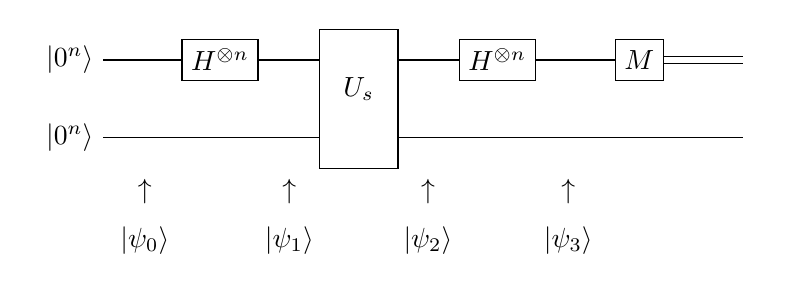
\begin{tikzpicture}%[thick]
	% `operator' will only be used by Hadamard (H) gates here.
	\tikzstyle{operator} = [draw,fill=white,minimum size=1.5em] 
	%
	\matrix[row sep=0.4cm, column sep=1cm] (circuit) {
		% First row
		\node (q1) {$\ket{0^n}$}; &
		\node[operator] (H11) {$H^{\otimes n}$}; &
		\node[operator] (P13) {}; &
		\node[operator] (H11) {$H^{\otimes n}$}; &
		\node[operator] (M11) {$M$};&
		\coordinate (end1); \\
		% Second row.
		\node (q2) {$\ket{0^n}$}; & & \node[operator] (P23) {}; & & & \coordinate (end2);\\
		% Third row
		\node (q31) {}; & \node (q32) {}; & \node (q33) {}; &
		\node (q34) {}; & \node (q35) {}; & \node (q36) {}; \\
		\node (q41) {}; & \node (q42) {}; & \node (q43) {}; &
		\node (q44) {}; & \node (q45) {}; & \node (q46) {}; \\
	};
	\node[operator] (Us) [fit = (P13) (P23), minimum width=1cm] {$U_s$};

	\node (arr0) [fit = (q31) (q32)] {$\uparrow$};
	\node (arr1) [fit = (q32) (q33)] {$\uparrow$};
	\node (arr2) [fit = (q33) (q34)] {$\uparrow$};
	\node (arr3) [fit = (q34) (q35)] {$\uparrow$};

	\node (psi0) [fit = (q41) (q42)] {$\ket{\psi_0}$};
	\node (psi1) [fit = (q42) (q43)] {$\ket{\psi_1}$};
	\node (psi2) [fit = (q43) (q44)] {$\ket{\psi_2}$};
	\node (psi3) [fit = (q44) (q45)] {$\ket{\psi_3}$};

	\node[fill=white, fit=(end1) (end2)] (cover) {};

	\begin{pgfonlayer}{background}
		% Draw lines.
		\draw (q1) -- (M11)  (q2) -- (end2);
		\draw[double, double distance=2pt] (M11) -- (end1);
	\end{pgfonlayer}

	%
	\end{tikzpicture}
\end{center}
%\end{figure}
Primero el sistema se inicia con ambas líneas a $\ket{0^n}$. Luego se aplica un 
operador de Hadamard sobre la primera, que creará una superposición de estados.  
Posteriormente, el operador $U_s$ computa los resultados de la función $f$ de 
forma simultánea. Para terminar, se revierte el operador de Hadamard sobre la 
primera línea, que finalmente se mide.

Los estados asociados a cada paso de la computación, han sido etiquetados como 
$\ket{\psi_i}$, de forma que en todo momento se pueda determinar el lugar al que 
corresponden en el circuito.

\subsection{Funcionamiento}
Para comprender el funcionamiento del algoritmo, se empleará un ejemplo sencillo 
con sólo dos bits, $n=2$ y de período $s=01$:
%
\begin{center}
\begin{tabular}{|c|c|}
	\hline
	$x$ & $f(x)$ \\
	\hline
	00 & 00 \\
	01 & 00 \\
	10 & 01 \\
	11 & 01 \\
	\hline
\end{tabular}
\end{center}
%
Sea $V = \{0,1\}^n$ entonces $f:V\rightarrow V$ y $f(x) = f(x\oplus s)$. De esta 
forma, $f(00) = f(00 \oplus s) = f(01)$ y también $f(10) = f(10 \oplus s) = 
f(11)$.

El sistema ha de iniciarse con ambas líneas a $\ket{0^n}$, de modo que:
%
$$ \ket{\psi_0} = \ket{0^n} \otimes \ket{0^n} $$
%
A continuación, el operador de Hadamard es aplicado sobre la línea superior.
%
\begin{equation}
\begin{split}
\ket{\psi_1} & = (H^{\otimes n} \otimes I^{\otimes n}) \ket{\phi_0} \\
	& = (H^{\otimes n} \otimes I^{\otimes n}) (\ket{0^n} \otimes \ket{0^n}) \\
	& = (H^{\otimes n} \ket{0^n}) \otimes (I^{\otimes n} \ket{0^n}) \\
	& = \frac{1}{\sqrt{2^n}} \sum_{x \in V} \ket{x, 00}
\end{split}
\end{equation}
%
Produciendo el estado entrelazado
%
\begin{equation}
\ket{\psi_1} = \frac{1}{\sqrt{2^2}} (\ket{00,00} + \ket{01,00} + \ket{10,00} + 
\ket{11,00})
\end{equation}
%
Posteriormente, la puerta $U_s$ actúa sobre $\ket{\psi_1}$ transformándolo en
%
\begin{equation}
\ket{\psi_2} = \frac{1}{\sqrt{2^n}} \sum_{x \in V} \ket{x, f(x) \oplus 00} = 
\frac{1}{\sqrt{2^n}} \sum_{x \in V} \ket{x, f(x)}
\end{equation}
%
En este estado, la función $f$ está siendo evaluada simultáneamente en todo $V$, 
y este efecto será clave para la reducción de complejidad. Con la función $f$ 
previamente descrita, dicho estado es
%
\begin{equation}
\ket{\psi_2} = \frac{1}{\sqrt{2^2}} (\ket{00,00} + \ket{01,00} + \ket{10,01} + 
\ket{11,01})
\end{equation}
%
Finalmente, el operador de Hadamard es nuevamente aplicado sobre la línea 
superior, de este modo se obtiene
% TODO: Explicar el origen de esta expresion
\begin{equation}
\ket{\psi_3} = \frac{1}{2^n} \sum_{x \in V} \sum_{z \in V}
	(-1)^{\braket{z|x}} \ket{z, f(x)}
\end{equation}
%
Por consiguiente, el coeficiente de cada ket será
%
\begin{equation}
c_k = \frac{1}{2^n} (-1)^{\braket{z|x}}
\end{equation}
%
Pero dado que $f(x) = f(x \oplus s)$, los kets $\ket{z, f(x)}$ y $\ket{z, f(x 
\oplus s)}$ serán el mismo, por lo que el coeficiente para este ket será
%
\begin{equation}
c_k = \frac{1}{2^n} \left((-1)^{\braket{z|x}} + (-1)^{\braket{z|x \oplus 
s}}\right)
\end{equation}
%
El producto interno $\braket{z|x \oplus s}$ puede descomponerse en $\braket{z|x} 
\oplus \braket{z|s}$, y substituyendo
%
\begin{equation}
\begin{split}
c_k & = \frac{1}{2^n} \left((-1)^{\braket{z|x}} + (-1)^{\braket{z|x} \oplus 
\braket{z|s}} \right) \\
	& = \frac{1}{2^n} \left((-1)^{\braket{z|x}} + (-1)^{\braket{z|x}}
	(-1)^{\braket{z|s}} \right)
\end{split}
\end{equation}
%
Cuando $\braket{z|s} = 1$, el coeficiente $c_k$ será
%
\begin{equation}
\begin{split}
c_k = \frac{1}{2^n} \left((-1)^{\braket{z|x}} - (-1)^{\braket{z|x}} \right) =
	\frac{1}{2^n} (0) = 0
\end{split}
\end{equation}
%
Y cuando $\braket{z|s} = 0$, será
%
\begin{equation}
c_k = \frac{1}{2^n} \left((-1)^{\braket{z|x}} + (-1)^{\braket{z|x}} \right)
	= \frac{1}{2^n} (\pm 2) = \pm 2^{1-n}
\end{equation}
%
De modo que $c_k \neq 0$ si en el ket $\ket{z, f(x)}$ se cumple que 
$\braket{z|s} = 0$. De modo que sólo los estados de la forma $\ket{z,y}$ tendrán 
coeficientes no nulos. En el caso del ejemplo será
%
\begin{equation}
\begin{split}
\ket{\psi_3} = 2^{-n} \big( &
		+ \ket{00,00} + \ket{01,00} + \ket{10,00} + \ket{11,00} \\
	& + \ket{00,00} - \ket{01,00} + \ket{10,00} - \ket{11,00} \\
	& + \ket{00,01} + \ket{01,01} - \ket{10,01} - \ket{11,01} \\
	& + \ket{00,01} - \ket{01,01} - \ket{10,01} + \ket{11,01}
	\big)
\end{split}
\end{equation}
%
Finalmente, tras anular los términos en los que $\braket{z|01} = 1$, es decir 
$z=01$ y $z=11$, queda
%
\begin{equation}
	\ket{\psi_3} = 2^{1-n} \left( \ket{00,00} + \ket{10,00} + \ket{00,01} - 
\ket{10,01} \right)
\end{equation}
%
En este estado, si se realiza una medición de $z$, el resultado siempre cumplirá 
la restricción $\braket{z|s} = 0$. Una vez que se obtengan $n-1$ vectores 
linealmente independientes, será posible construir un sistema de ecuaciones y 
calcular $s$.

En este ejemplo, después de medir la primera línea, el conjunto de vectores 
posibles resulta $z \in \{00, 10\}$. En todo caso, se tiene que $\braket{z|s} = 
0$ de modo que $\braket{00|s} = 0$ y $\braket{10|s} = 0$, produciendo las 
ecuaciones:
%
\begin{equation}
\begin{split}
	0 s_0 \oplus 0 s_1 = 0 \\
	1 s_0 \oplus 0 s_1 = 0
\end{split}
\end{equation}
%
Cuyas soluciones son $s \in \{00, 01\}$, pero dado que $s \neq 00$, se obtiene 
$s = 01$.














\end{document}


\end
